% XCircuit output "multiplicador.tex" for LaTeX input from multiplicador.eps
\def\putbox#1#2#3#4{\makebox[0in][l]{\makebox[#1][l]{}\raisebox{\baselineskip}[0in][0in]{\raisebox{#2}[0in][0in]{\scalebox{#3}{#4}}}}}
\def\rightbox#1{\makebox[0in][r]{#1}}
\def\centbox#1{\makebox[0in]{#1}}
\def\topbox#1{\raisebox{-0.60\baselineskip}[0in][0in]{#1}}
\def\midbox#1{\raisebox{-0.20\baselineskip}[0in][0in]{#1}}
   \scalebox{1}{
   \normalsize
   \parbox{4.18229in}{
   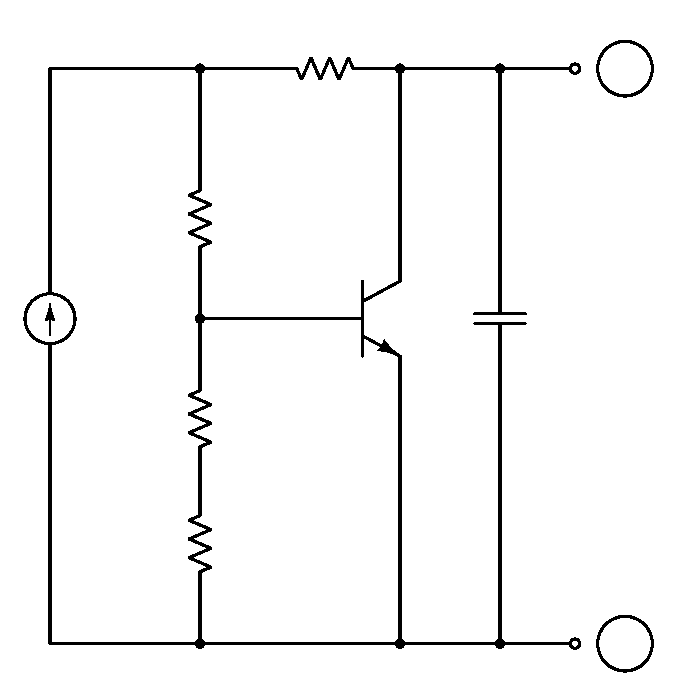
\includegraphics[scale=1]{multiplicador}\\
   % translate x=672 y=611 scale 0.38
   \putbox{3.56in}{2.32in}{1.20}{CM}%
   \putbox{2.47in}{2.32in}{1.20}{QM}%
   \putbox{0.56in}{3.07in}{1.20}{R1M}%
   \putbox{0.72in}{1.74in}{1.20}{Rp}%
   \putbox{0.64in}{0.82in}{1.20}{R2M}%
   \putbox{1.89in}{4.24in}{1.20}{R3M}%
   \putbox{4.06in}{4.07in}{1.20}{\centbox{\midbox{1,1}}}%
   \putbox{4.06in}{0.24in}{1.20}{\centbox{\midbox{-1,1}}}%
   \putbox{0.47in}{2.32in}{1.20}{Ipol}%
   \putbox{1.97in}{3.74in}{1.20}{$10 \Omega$}%
   \putbox{1.47in}{3.07in}{1.20}{$3,3 k\Omega$}%
   \putbox{1.39in}{0.82in}{1.20}{$680 \Omega$}%
   \putbox{1.39in}{1.65in}{1.20}{$1 k\Omega$}%
   } % close 'parbox'
   } % close 'scalebox'
   \vspace{-\baselineskip} % this is not necessary, but looks better
